% !TEX encoding = UTF-8
% !TEX TS-program = pdflatex
% !TEX root = ../tesi.tex

%**************************************************************
\chapter{Analisi dei requisiti}
\label{cap:analisi-requisiti}
%**************************************************************

\intro{In questo capitolo vengono definite con precisione le funzionalità del software che è stato prodotto durante lo stage. Viene presentata l'analisi dei requisiti svolta per il progetto, approfondita con i diagrammi dei casi d'uso.}\\

\section{Casi d'uso}
I diagrammi dei casi d'uso (in inglese, \textit{Use Case Diagram}) sono diagrammi di tipo \gls{umlg} che servono a descrivere le interazioni fra il sistema software e gli utenti che lo utilizzano, mostrando l'insieme funzionalità esposte dal sistema dal punto di vista degli utenti. \\
Poiché lo stage era incentrato sull'estensione del framework e lo sviluppo di un algoritmo euristico per la risoluzione dei problemi di scheduling, la prima parte del progetto non necessitava di esporre funzionalità all'utente. D'altro canto, una volta sviluppata l'applicazione per risolvere il problema specifico del casinò, avrei dovuto garantire dei servizi minimi all'utente per inserire l'input (informazioni circa le postazioni, i lavoratori, i turni) e mostrare l'output (lo scheduling prodotto). \\
Per questo motivo i diagrammi dei casi d'uso risultano minimali e in numero ridotto.\\
\\
Ogni caso d'uso è classificato secondo la seguente convenzione:
\begin{center}
    UC[Codice padre]*.[Codice identificativo]
\end{center}

\begin{itemize}
    \item \textbf{Codice padre}: \MakeUppercase{} il codice identificativo del caso d'uso generico che ha generato il caso d'uso in esame. Se il caso d'uso non è stato generato da altri, va tralasciato;
    \item \textbf{Codice identificativo}: Identifica univocamente il caso d'uso. \MakeUppercase{è} un codice composto da sole cifre. 
\end{itemize}
\noindent
Alcuni casi d'uso possono essere associati ad un diagramma dei casi d'uso riportante lo stesso titolo e codice.
\clearpage
\subsection{Diagrammi dei casi d'uso}
La \hyperref[fig41]{Figura 4.1} presenta il diagramma dei casi d'uso generale.
\begin{figure}[!h]
    \begin{widepage}
        \label{fig41}
        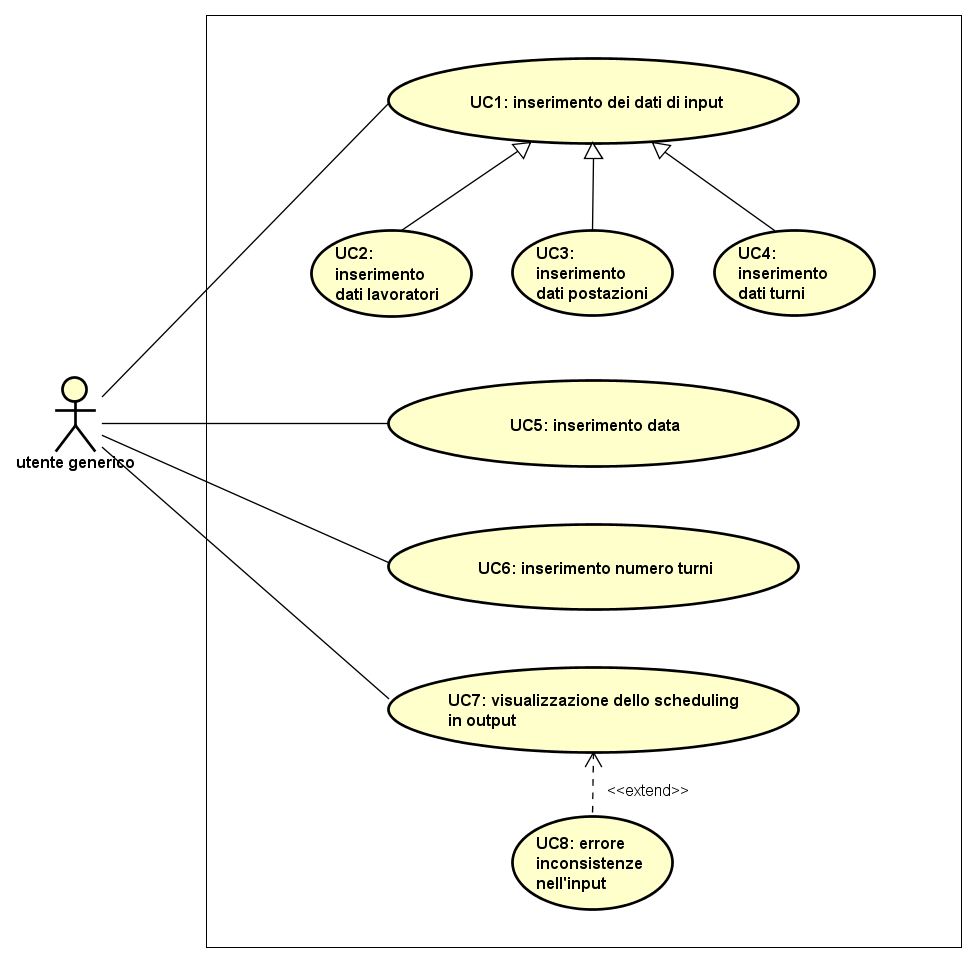
\includegraphics[width=\textwidth,keepaspectratio]{../immagini/usecase/System.png}
        \caption{Diagramma dei casi d'uso ad alto livello}
    \end{widepage}
\end{figure}
\clearpage
\subsection{UC1: Inserimento dei dati di input}
\label{UC1}
\begin{itemize}
    \item \textbf{Attori}: utente generico;
    \item \textbf{Descrizione}: l'utente inserisce i dati in input al programma per realizzare uno scheduling.
    \item \textbf{Generalizzazioni}: l'utente inserisce i dati in input al programma per realizzare uno scheduling riguardati i lavoratori (UC2), le postazioni (UC3), i turni (UC4).
\end{itemize}

\subsection{UC2: Inserimento dati lavoratori}
\label{UC2}
La \hyperref[fig42]{Figura 4.2} presenta il diagramma dei casi d'uso relativo all'UC2.
\begin{figure}[!h]
    \begin{widepage}
        \label{fig42}
    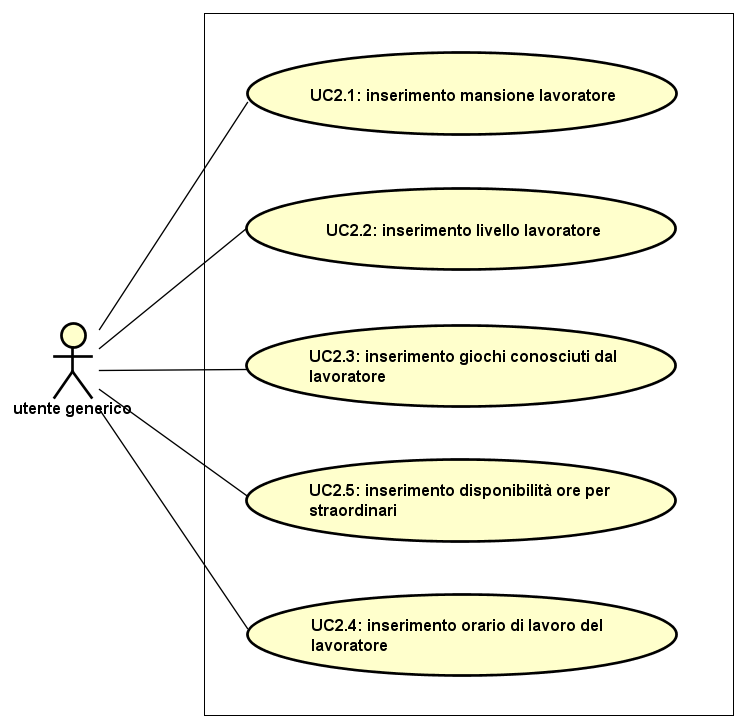
\includegraphics[width=14.9cm,keepaspectratio]{../immagini/usecase/UC2.png}
    \caption{UC2: Inserimento dati lavoratori}
    \end{widepage}
\end{figure}
\clearpage
\begin{itemize}
    \item \textbf{Attori}: utente generico;
    \item \textbf{Descrizione}: l'utente inserisce i dati in input al programma per realizzare uno scheduling riguardanti i lavoratori.
\end{itemize}
\paragraph{UC2.1: Inserimento mansione lavoratore}
\begin{itemize}
    \item \textbf{Attori}: utente generico;
    \item \textbf{Descrizione}: l'utente inserisce i dati in input al programma circa la mansione del lavoratore (dealer, dealer-inspector, inspector).
\end{itemize}
\paragraph{UC2.2: Inserimento livello lavoratore}
\begin{itemize}
    \item \textbf{Attori}: utente generico;
    \item \textbf{Descrizione}: l'utente inserisce i dati in input al programma circa il livello del lavoratore (dealer: 1-8, dealer-inspector: 3, inspector: 1-3).
\end{itemize}
\paragraph{UC2.3: Inserimento giochi conosciuti dal lavoratore}
\begin{itemize}
    \item \textbf{Attori}: utente generico;
    \item \textbf{Descrizione}: l'utente inserisce i dati in input al programma circa i giochi conosciuti dal lavoratore.
\end{itemize}
\paragraph{UC2.4: Inserimento orario di lavoro del lavoratore}
\begin{itemize}
    \item \textbf{Attori}: utente generico;
    \item \textbf{Descrizione}: l'utente inserisce i dati in input al programma circa l'orario di lavoro del giocatore (ora di inizio, ora di fine).
\end{itemize}
\paragraph{UC2.5: Inserimento disponibilità ore per straordinari}
\begin{itemize}
    \item \textbf{Attori}: utente generico;
    \item \textbf{Descrizione}: l'utente inserisce i dati in input al programma circa la disponibilità a svolgere straordinari (ore).
\end{itemize}
\clearpage
\subsection{UC3: Inserimento dati postazioni}
\label{UC3}
La \hyperref[fig43]{Figura 4.3} presenta il diagramma dei casi d'uso relativo all'UC3.
\begin{figure}[!h]
    \label{fig43}
    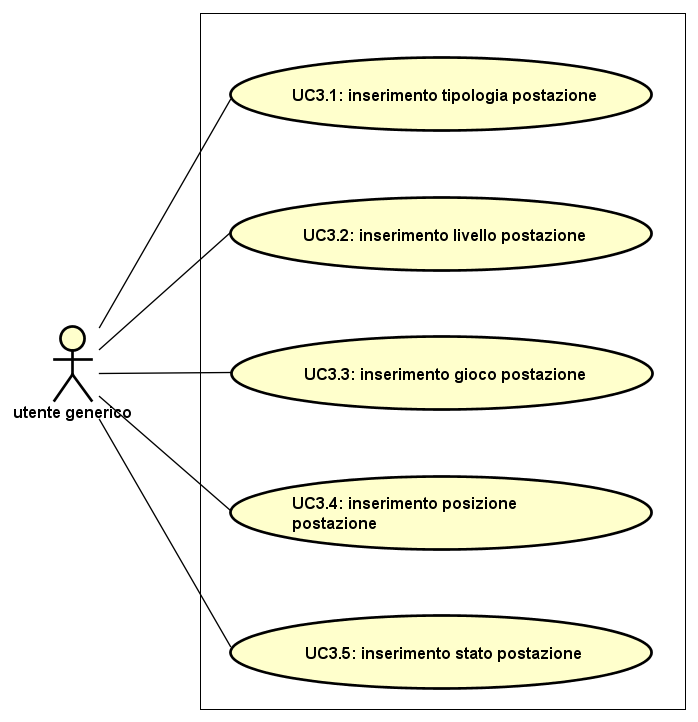
\includegraphics[width=\textwidth]{../immagini/usecase/UC3.png}
    \caption{UC3: Inserimento dati postazioni}
\end{figure}
\FloatBarrier
\noindent
\begin{itemize}
    \item \textbf{Attori}: utente generico;
    \item \textbf{Descrizione}: l'utente inserisce i dati in input al programma per realizzare uno scheduling riguardanti le postazioni.
\end{itemize}
\paragraph{UC3.1: Inserimento tipologia postazione}
\begin{itemize}
    \item \textbf{Attori}: utente generico;
    \item \textbf{Descrizione}: l'utente inserisce i dati in input al programma circa la tipologia della postazione (tavolo, pit).
\end{itemize}
\paragraph{UC3.2: Inserimento livello postazione}
\begin{itemize}
    \item \textbf{Attori}: utente generico;
    \item \textbf{Descrizione}: l'utente inserisce i dati in input al programma circa il livello della postazione (tavoli: 1-8, pit: 1-3).
\end{itemize}
\paragraph{UC3.3: Inserimento gioco postazione}
\begin{itemize}
    \item \textbf{Attori}: utente generico;
    \item \textbf{Descrizione}: l'utente inserisce i dati in input al programma circa il gioco che si gioca nella postazione.
\end{itemize}
\paragraph{UC3.4: Inserimento posizione postazione}
\begin{itemize}
    \item \textbf{Attori}: utente generico;
    \item \textbf{Descrizione}: l'utente inserisce i dati in input al programma circa la posizione che si assume lavorando nella postazione (seduta, in piedi).
\end{itemize}
\paragraph{UC3.5: Inserimento stato}
\begin{itemize}
    \item \textbf{Attori}: utente generico;
    \item \textbf{Descrizione}: l'utente inserisce i dati in input al programma circa lo stato della postazione (aperta, chiusa).
\end{itemize}
\subsection{UC4: Inserimento dati turni}
\label{UC4}
La \hyperref[fig44]{Figura 4.4} presenta il diagramma dei casi d'uso relativo all'UC4.
\begin{figure}[!h]
    \label{fig44}
    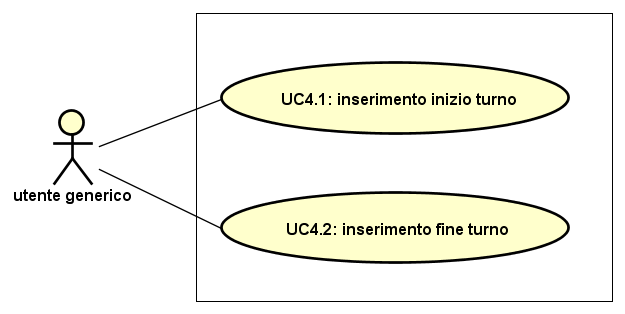
\includegraphics[width=\textwidth]{../immagini/usecase/UC4.png}
    \caption{UC4: Inserimento dati turni}
\end{figure}
\FloatBarrier
\noindent
\begin{itemize}
    \item \textbf{Attori}: utente generico;
    \item \textbf{Descrizione}: l'utente inserisce i dati in input al programma per realizzare uno scheduling riguardanti i turni.
\end{itemize}
\paragraph{UC4.1: Inserimento inizio turno}
\begin{itemize}
\item \textbf{Attori}: utente generico;
\item \textbf{Descrizione}: l'utente inserisce i dati in input al programma circa l'ora di inizio di un turno.
\end{itemize}
\paragraph{UC4.2: Inserimento fine turno}
\begin{itemize}
\item \textbf{Attori}: utente generico;
\item \textbf{Descrizione}: l'utente inserisce i dati in input al programma circa l'ora di fine di un turno.
\end{itemize}

\subsection{UC5: Inserimento data}
\label{UC5}
\begin{itemize}
    \item \textbf{Attori}: utente generico;
    \item \textbf{Descrizione}: l'utente inserisce la data per la quale vuole trovare uno scheduling (importante perché gli orari del personale possono variare di data in data).
    \item \textbf{Scenario alternativo}: se l'utente non inserisce una data, viene trovato lo scheduling per il giorno corrente.
\end{itemize}

\subsection{UC6: Inserimento numero turni}
\label{UC6}
\begin{itemize}
    \item \textbf{Attori}: utente generico;
    \item \textbf{Descrizione}: l'utente inserisce il numero di turni per il quale vuole trovare uno scheduling.
    \item \textbf{Scenario alternativo}: se l'utente non inserisce un numero, viene trovato lo scheduling per tutti i turni.
\end{itemize}

\subsection{UC7: Visualizzazione dello scheduling in output}
\label{UC7}
\begin{itemize}
    \item \textbf{Attori}: utente generico;
    \item \textbf{Descrizione}: l'utente visualizza l'output del programma (soluzione ammissibile o non).
    \item \textbf{Estensioni}: non c'è output perché è stato commesso un errore di inserimento dei dati.
\end{itemize}
\clearpage
%***********************************************************************
\section{Requisiti}

Sono riportati di seguito i requisiti individuati per il progetto con rispettivo codice identificativo, importanza e breve descrizione.
\newline
\begin{itemize}
    \item \textbf{Codice identificativo:} \`e la sigla che identifica ogni requisito e rispetta la seguente notazione:
    \begin{center}
        R[Tipo][Importanza][Identificativo]
    \end{center}
    \textbf{Tipo:}
    \begin{itemize}
        \item \textbf{F:} requisito funzionale;
        \item \textbf{V:} requisito di vincolo;
        \item \textbf{Q:} requisito qualitativo;
    \end{itemize}
    \textbf{Importanza:}
    \begin{itemize}
        \item \textbf{O:} requisito obbligatorio;
        \item \textbf{D:} requisito desiderabile;
        \item \textbf{F:} requisito opzionale.
    \end{itemize}
    \textbf{Identificativo:} codice che identifica in modo univoco un requisito. Viene rappresentato con la notazione decimale puntata per rendere pi\`u intuibile la forma gerarchica.
    \item \textbf{Descrizione:} indica testualmente la necessit\`a rappresentata dal requisito.
\end{itemize}
\noindent
Nel paragrafo ``\hyperref[setteuno]{7.1 - Raggiungimento degli obiettivi}''
è presente un consuntivo che riporta quanti dei requisiti elencati di seguito sono stati soddisfatti nel corso dello stage.

\subsection{Requisiti Funzionali}
I requisiti funzionali sono indicati nella \hyperref[tab:req-fun-fr]{Tabella 4.1}.
\begin{table}[!h]
    \caption{Tabella dei requisiti funzionali}
    \label{tab:req-fun-fr}
    \begin{tabularx}{\textwidth}{|c|c|X|}
        \hline
        \thead{ID} & \thead{Importanza} & \thead{Descrizione}\\
        \hline \hline
        RFO1 & Obbligatorio & L'utente deve poter fornire l'input al programma. \\ \hline
        RFO1.1 & Obbligatorio & L'utente deve poter fornire l'input circa gli \items\ al programma. \\ \hline
        RFO1.2 & Obbligatorio & L'utente deve poter fornire l'input circa i \task\ al programma. \\ \hline
        RFO1.3 & Obbligatorio & L'utente deve poter fornire l'input circa i \ttb\ al programma. \\ \hline    
    \end{tabularx}
\end{table}%

\begin{table}[!h]
    \begin{tabularx}{\textwidth}{|c|c|X|}
        \hline
        \thead{ID} & \thead{Importanza} & \thead{Descrizione}\\
        \hline \hline
            RFO2 & Obbligatorio & Il programma deve poter caricare l'input fornito dall'utente.\\ \hline
            RFO2.1 & Obbligatorio & Se l'input non è corretto, il{\tiny } programma deve dare un messaggio di errore.\\ \hline
            
            RFO3 & Obbligatorio & L'utente deve scegliere la data per cui eseguire lo scheduling.\\ \hline
            
            RFD4 & Desiderabile & L'utente deve poter bloccare la produzione dello scheduling dopo un certo numero di turni.\\ \hline
            
            RFO5 & Obbligatorio & Il programma deve dedurre da che \ttb\ cominciare lo scheduling.\\ \hline
            RFO5.1 & Obbligatorio & Se l'utente vuole produrre uno scheduling per un giorno diverso dal corrente, lo scheduling va cominciato dal primo \ttb.\\ \hline
            RFO5.2 & Obbligatorio & Se l'utente vuole produrre uno scheduling per il giorno corrente e l'orario di inizio del primo \ttb\ non è ancora arrivato, lo scheduling va cominciato dal primo \ttb.\\ \hline
            RFO5.3 & Obbligatorio & Se l'utente vuole produrre uno scheduling per il giorno corrente e i \ttb\ sono già cominciati, lo scheduling va cominciato dal \ttb\ successivo al corrente.\\ \hline
            
            RFO6 & Obbligatorio & Il programma deve produrre uno scheduling rispettando i vincoli imposti dal problema.\\ \hline
            
            RFO7 & Obbligatorio & Il programma deve produrre uno scheduling fair.\\ \hline
            
            RFO8 & Obbligatorio & Se non esiste una soluzione ammissibile, il programma deve comunque fornirne una con l'ausilio del Dummy Worker.\\ \hline
            
            RFO9 & Obbligatorio & Il programma deve compiere delle iterazioni migliorative e fornire più di uno scheduling.\\ \hline
            RFO9.1 & Obbligatorio & Le iterazioni sono considerate migliorative se riducono il costo degli \items.\\ \hline
            
            RFO10 & Obbligatorio & Il programma deve essere flessibile circa la disponibilità dei \task. \\ \hline
    \end{tabularx}
\end{table}%
\clearpage
\begin{table}[!h]
    \begin{tabularx}{\textwidth}{|c|c|X|}
        \hline
        \thead{ID} & \thead{Importanza} & \thead{Descrizione}\\
        \hline \hline
        RFO11 & Obbligatorio & Il programma deve essere flessibile circa la disponibilità degli \items. \\ \hline
         
        RFO12 & Obbligatorio & Il programma deve creare un output per l'utente con gli scheduling prodotti. \\ \hline
        
        RFO13 & Obbligatorio & Il programma deve creare un output per l'utente con gli scheduling prodotti. \\ \hline
        
        RFF14 & Opzionale & Gli output devono avere facilitazioni all'uso per l'utente. \\ \hline
        RFF14.1 & Opzionale & L'utente deve poter individuare facilmente le assegnazioni dello stesso \task. \\ \hline
    \end{tabularx}
\end{table}%
\clearpage
\subsection{Requisiti di Qualità}
I requisiti di qualità sono indicati nella \hyperref[tab:req-q]{Tabella 4.2}.
\begin{table}[!h]
    \caption{Tabella dei requisiti di qualità}
    \label{tab:req-q}
    \begin{tabularx}{\textwidth}{|c|c|X|}
        \hline
        \thead{ID} & \thead{Importanza} & \thead{Descrizione}\\
        \hline \hline
        RQO1 & Obbligatorio & Deve essere fornito il manuale dello sviluppatore che descrive classi, metodi e funzionamento del software.\\
        \hline
        RQO2 & Obbligatorio & Deve essere fornito il manuale utente
        per aiutare l'utente nell'utilizzo
        dell'applicazione.\\
        \hline
        RQO3 & Obbligatorio & Devono essere fornite relazioni tecniche circa gli studi svolti.\\
        \hline
        RQO4 & Obbligatorio & Devono essere fornite relazioni tecniche circa i risultati ottenuti.\\
        \hline
        RQD5 & Desiderabile & Deve essere fornita una relazione circa l'esplorazione di altri contesti applicativi.\\
        \hline
    \end{tabularx}
\end{table}%
\FloatBarrier
\subsection{Requisiti di Vincolo}
I requisiti di vincolo sono indicati nella \hyperref[tab:req-vin]{Tabella 4.3}.
\begin{table}[!h]
    \caption{Tabella dei requisiti di vincolo}
    \label{tab:req-vin}
    \begin{tabularx}{\textwidth}{|c|c|X|}
        \hline
        \thead{ID} & \thead{Importanza} & \thead{Descrizione}\\
        \hline \hline
        RVO1 & Obbligatorio & Il framework per la risoluzione dei problemi di scheduling deve andare ad integrarsi al framework aziendale.\\
        \hline
        RVO2 & Obbligatorio & Il problema di scheduling specifico deve essere risolto utilizzando il framework aziendale esteso.\\
        \hline
        RVO3 & Obbligatorio & L'input e l'output devono esere gestiti tramite file xls.\\
        \hline
        RVF4 & Opzionale & Visualizzazione dell'output tramite HTML.\\
        \hline 
        RVF5 & Opzionale & Il modello deve essere implementato in AMPL.\\
        \hline
    \end{tabularx}
\end{table}%